\chapter{Progettazione della Soluzione}
\section{Class Diagram del dominio della soluzione}
	\begin{figure}[hbt]
	\centering
  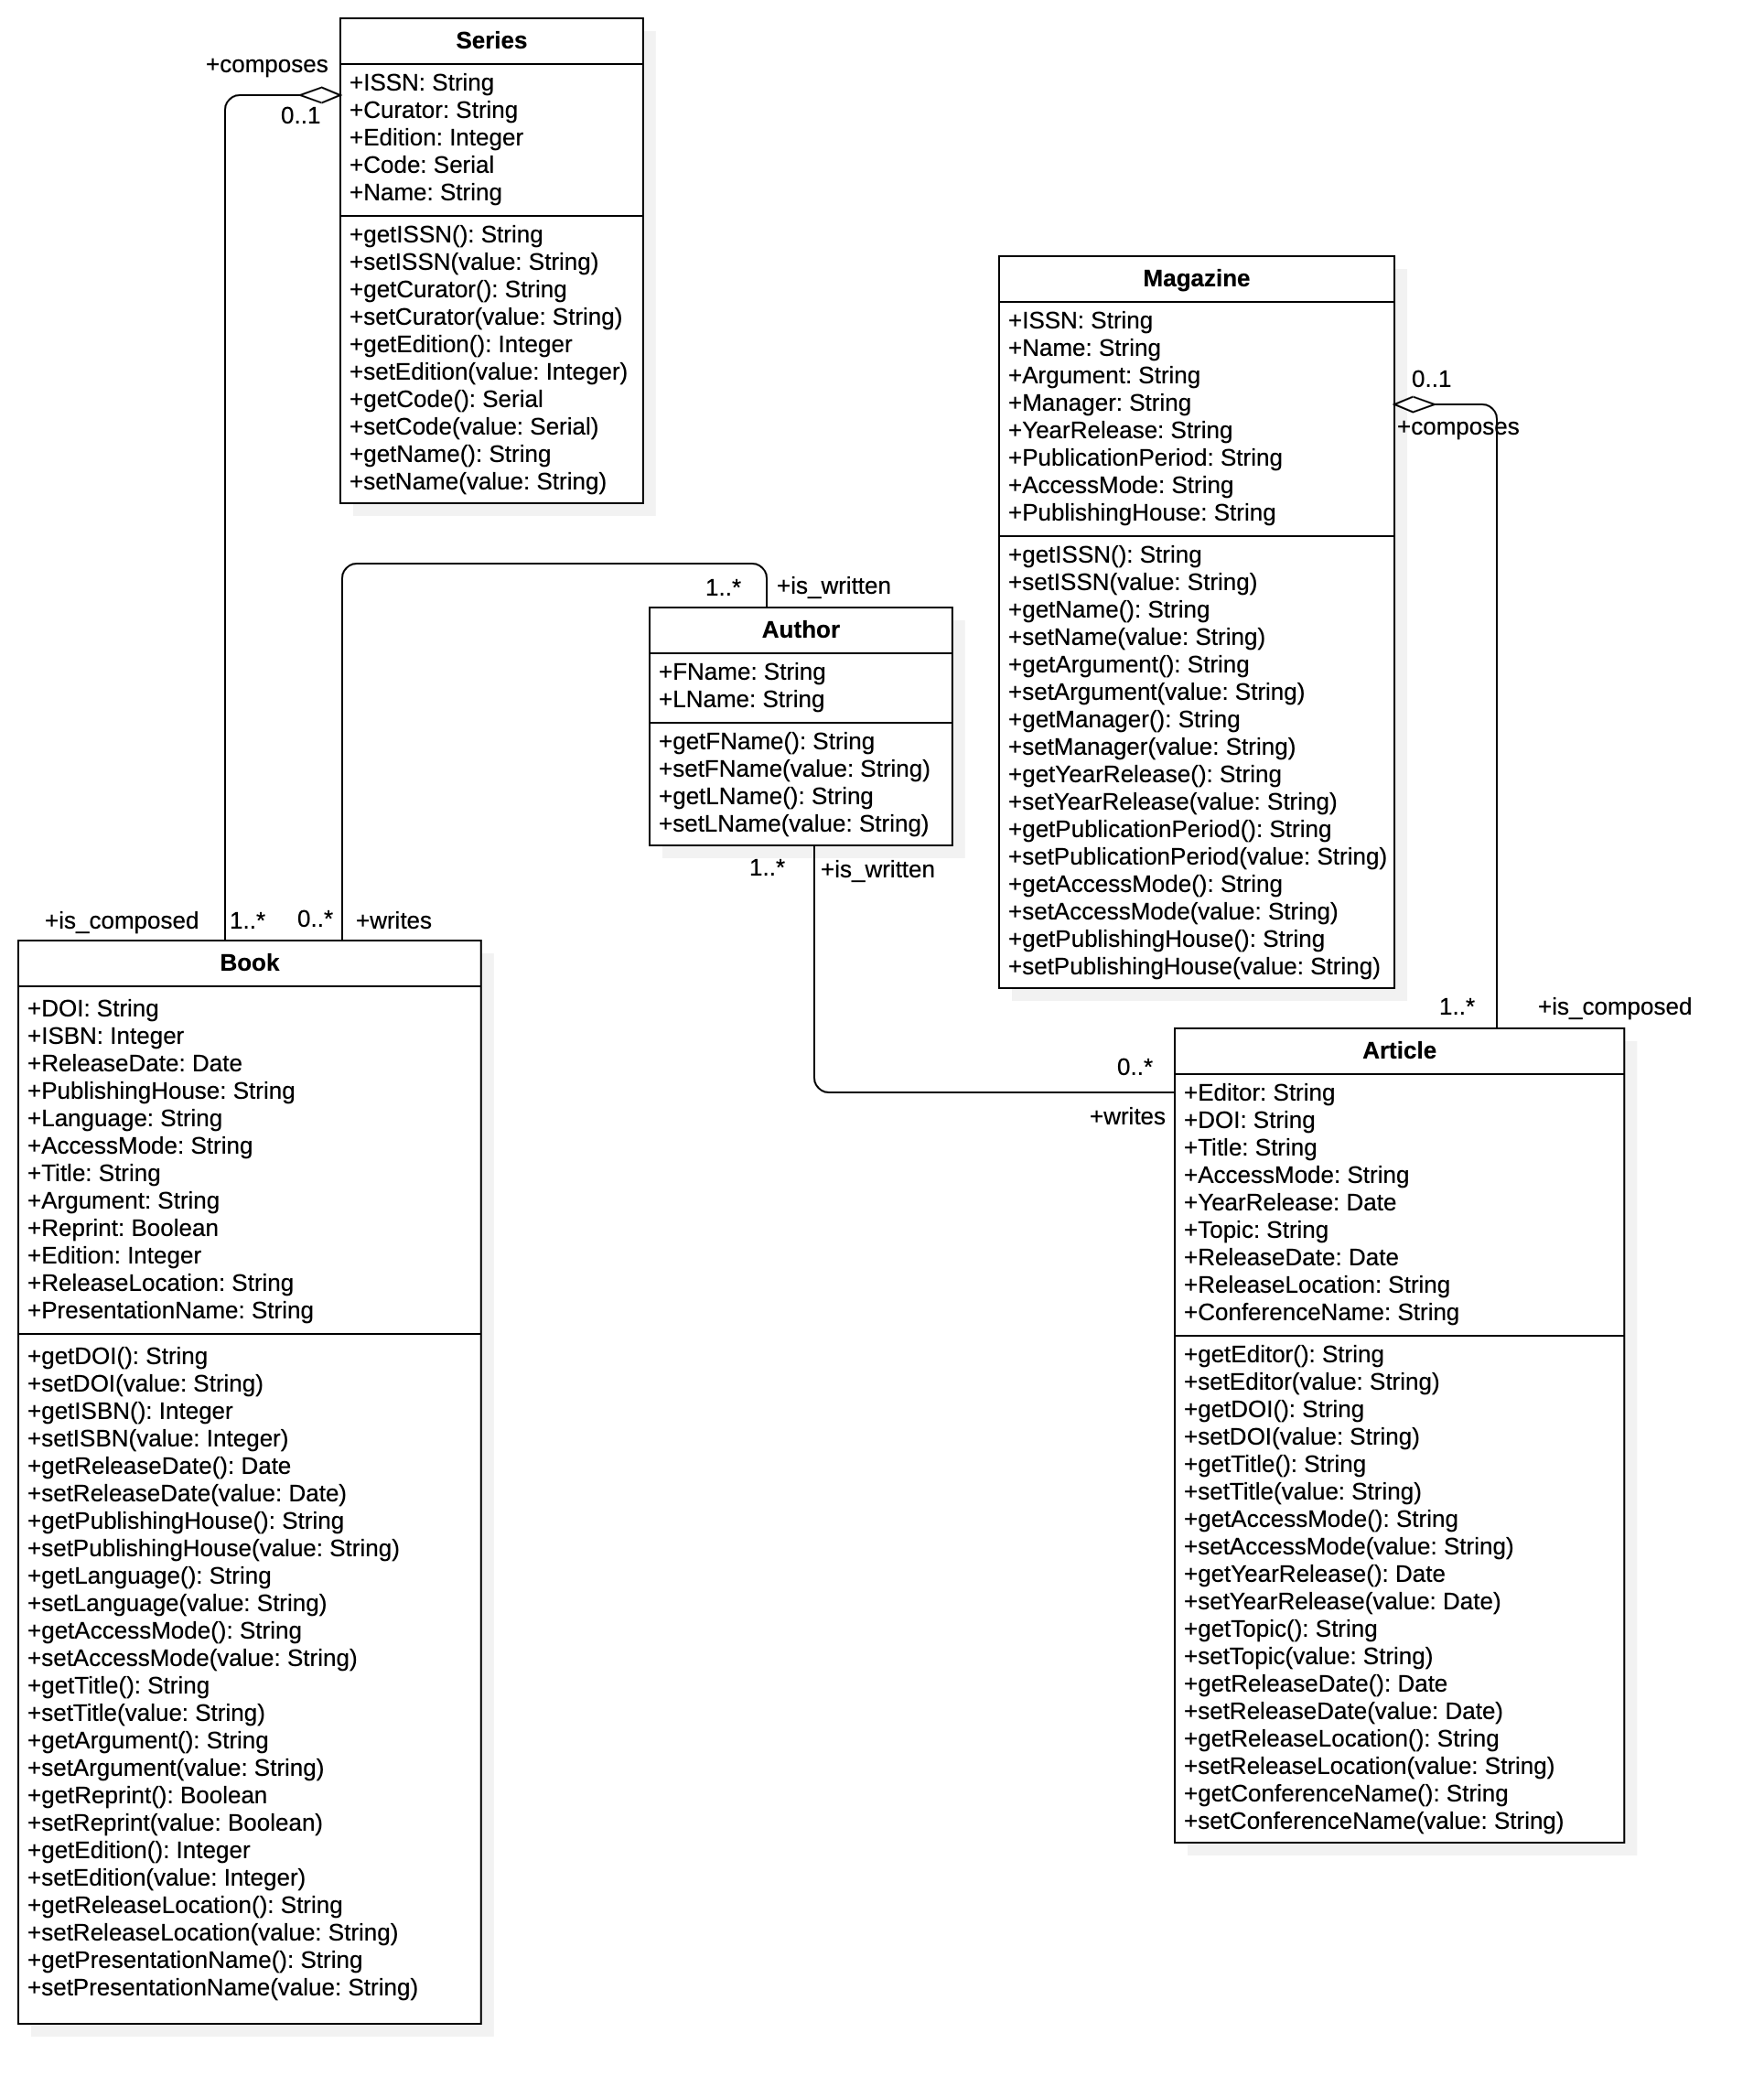
\includegraphics[width=0.7\textwidth]{/Users/lorenzotecchia/Documents/ESAMI/ProgettoOOBD/OO/Documentazione/Diagrammi/ClassDiagramS.png}
  \caption{Class Diagram del dominio della soluzione}
\end{figure}


\begin{table}[]
	\section{Dizionario dei metodi}
\centering
\caption{Dizionario dei Metodi}
\label{tab:DizionarioMetodi}
\resizebox{\textwidth}{!}{%
\begin{tabular}{|l|l|}
\hline
\rowcolor[HTML]{762DC3} 
Classe &
  Metodi \\ \hline
Series &
  \begin{tabular}[c]{@{}l@{}}+getISSN(): String +setISSN(value: String)\\ +getCurator(): String +setCurator(value: String)\\ +getEdition(): Integer +setEdition(value: Integer)\\ +getCode(): Serial +setCode (value: Serial)\\ +getName(): String +setName (value: String)\end{tabular} \\ \hline
Author &
  \begin{tabular}[c]{@{}l@{}}+getFName(): String +setFName(value: String)\\ +getLName(): String + setLName(value: String)\end{tabular} \\ \hline
Magazine &
  \begin{tabular}[c]{@{}l@{}}+getISSN(): String +setISSN(value: String)\\ +getName(): String +setName(value: String)\\ +getArgument(): String +setArgument(value: String)\\ +getManager(): String +setManager(value: String)\\ +getYearRelease: String +setYearRelease(value: String)\\ +getPublicationPeriod(): String +setPublicationPeriod(value: String)\\ +getAccessMode(): String +setAccessMode(value: String)\\ +getPublishingHouse(): String +setPublishingHouse(value: String)\end{tabular} \\ \hline
Article &
  \begin{tabular}[c]{@{}l@{}}+getEditor(): String +setEditor(value: String) \\ +getDOI(): String +setDOl(value: String) \\ +getTitle(): String +setTitle(value: String) \\ +getAccessMode(): String +setAccessMode(value: String) \\ +getYearRelease(): Date +setYearRelease (value: Date) \\ +getTopic(): String +setTopic(value: String) \\ +getReleaseDate(): Date +setReleaseDate (value: Date) \\ +getReleaseLocation(): String +setReleaseLocation(value: String) \\ +getConferenceName(): String +setConferenceName(value: String)\end{tabular} \\ \hline
Book &
  \begin{tabular}[c]{@{}l@{}}+getDOI0: String +setDOl(value: String)\\ +getISBN(): Integer +setISBN(value: Integer) \\ +getReleaseDate(): Date +setReleaseDate(value: Date) \\ +getPublishingHouse(): String +setPublishingHouse(value: String) \\ +getLanguage(): String +setLanguage(value: String) \\ +getAccessMode(): String +setAccessMode(value: String) \\ +getTitle(): String +setTitle(value: String) \\ +getArgument(): String +setArgument(value: String) \\ +getReprint(): Boolean +setReprint(value: Boolean) \\ +getEdition(): Integer +setEdition(value: Integer) \\ +getReleaseLocation(): String +setReleaseLocation(value: String) \\ +getPresentationName(): String +setPresentationName(value: String)\end{tabular} \\ \hline
\end{tabular}%
}
\end{table}
	
	\section{Sequence Diagram del metodo $\rightarrow$ Primo metodo}
	\section{Sequence Diagram del metodo $\rightarrow$ Secondo metodo}